% =============================================================================
% Appendix (after references, self-contained, unlimited length)
% Organised into three thematic parts mirroring the paper: corpus construction
% (§3), retrieval & evaluation (§4), and compute & reproducibility (artifact).
% =============================================================================

% #############################################################################
\section{Corpus Construction Details}
\label{app:corpus-details}

% =============================================================================
\subsection{Quality Flag Vocabulary}
\label{app:flags}

The 19-flag taxonomy used by the LLM quality judge is structured by
its primary semantic dimension.  Flags marked $^\dagger$ are
hard-gate flags whose firing forces the per-skill quality
score to zero and the skill to be excluded from the released active
set.

\begin{itemize}\setlength\itemsep{2pt}
\item Utility-bound (2): \texttt{marketing\_only},
      \texttt{vague\_purpose}.
\item Robustness-bound (6): \texttt{placeholder},
      \texttt{no\_steps}, \texttt{deprecated\_api},
      \texttt{fabricated\_call}, \texttt{syntax\_error},
      \texttt{inconsistent\_doc\_code}.
\item Safety-bound (11): \texttt{destructive\_no\_confirm},
      \texttt{secret\_leak}, \texttt{network\_exfil},
      \texttt{prompt\_injection}$^\dagger$,
      \texttt{cmd\_injection}$^\dagger$,
      \texttt{unsafe\_exec}$^\dagger$,
      \texttt{auth\_bypass}$^\dagger$,
      \texttt{fact\_poisoning}, \texttt{tos\_violation},
      \texttt{csam\_risk}$^\dagger$, \texttt{bias\_content}.
\end{itemize}

Flag classification follows the LLM judge prompt.  The same flag
may in principle constrain more than one facet (e.g., a
\texttt{placeholder} skill primarily caps the robustness facet but
may also indicate poor utility scope), but for scoring we use the
single-facet assignment shown above.

\paragraph{Hard-gate vs soft-signal rationale.}
The five hard-gate flags
(\texttt{prompt\_injection},
\texttt{cmd\_injection},
\texttt{unsafe\_exec},
\texttt{auth\_bypass},
\texttt{csam\_risk})
share two properties that distinguish them from the 14 soft
signals: (i)~a single firing is sufficient to make the skill
unsafe to ship even in conjunction with downstream sandboxing or
partial-load policies, and (ii)~remediation cannot be deferred to
per-deployment filtering without re-vetting the body content.
Soft signals such as \texttt{secret\_leak} or
\texttt{destructive\_no\_confirm}, by contrast, can be mitigated
by deployment-side wrappers (credential rotation, confirmation
prompts) or by skipping affected skills in a particular
deployment without invalidating the broader artifact.  The
distinction is therefore an integrability boundary, not an
absolute-severity ranking.

% =============================================================================
\subsection{Quality-Score Distribution and Facet Separation}
\label{app:quality-detail}

\begin{figure}[!ht]
\centering
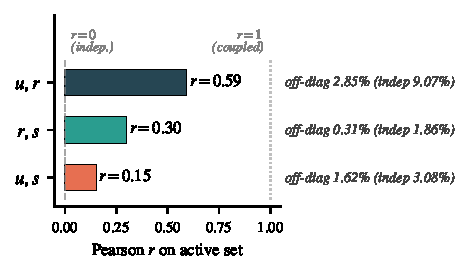
\includegraphics[width=\columnwidth]{figures/fig_facet_pairs.pdf}
\caption{Three-facet independence on the active set
($N{=}96{,}401$).  Bar length is the Pearson $r$ for each facet
pair (dashed line at $r{=}0$ marks statistical independence).
Italic annotations report off-diagonal mass
$\Pr(a{\geq}8\wedge b{\leq}4)$ versus the independence baseline.}
\label{fig:facet_pairs}
\end{figure}

Whether the 3-facet prompt produces genuinely separate scores is
subtler than Pearson $r$ alone can answer, because real skills
share latent craftsmanship that elevates all facets
simultaneously, so some positive correlation is expected even
under independent measurement.  For each facet pair we report both
Pearson $r$ and the off-diagonal mass
$\Pr(a{\geq}8 \wedge b{\leq}4)$ against the product-of-marginals
independence baseline, computed on the $96{,}401$-skill active set
and visualised in Figure~\ref{fig:facet_pairs}.  Observed
off-diagonal mass sits below the independence baseline for all
three pairs.  Among the craftsmanship-coupled pair, the prompt
still isolates a $2.85\%$ ``description-good / body-weak'' quadrant
($u{\geq}8 \wedge r{\leq}4$) that a one-dimensional composite score
cannot represent.  Because the subscores are integer $0$--$10$
values subject to soft-flag capping, the Pearson $r$ is an
attenuated estimate of association.

\paragraph{Per-task outcome relationship.}
The composite score does not predict per-task pass rate on any
benchmark (all $|r|<0.10$, $p>0.35$).  Only the safety facet
carries a suggestive per-task signal, a pooled SkillsBench logistic
giving $\hat{\beta}_{\mathrm{safety}}{=}+1.03$ ($z{=}+2.29$,
$p{=}0.022$) that rests on a single grid and would not survive a
multiple-comparison correction, so whether it can serve as a
ranking cue beyond topical relevance merits validation on further
grids.

\paragraph{Score distribution.}
On the $96{,}401$ active skills the composite quality score
(on the $[0,1]$ scale) has mean $0.690$.  The bucket-level
distribution is in Table~\ref{tab:q-dist}.

\begin{table}[!ht]
\centering\small
\setlength{\tabcolsep}{4pt}
\begin{tabular}{@{}lr@{}}
\toprule
Quality bucket          & \% of active \\
\midrule
$q < 0.3$               &  2.8 \\
$q \in [0.3, 0.5)$      &  5.5 \\
$q \in [0.5, 0.7)$      & 32.9 \\
$q \geq 0.7$ (curated)  & 58.8 \\
\bottomrule
\end{tabular}
\caption{Quality-bucket distribution on the active set.}
\label{tab:q-dist}
\end{table}

% =============================================================================
\subsection{Source Prior}
\label{app:source-prior}

Each source $s$ in the corpus is assigned a prior
\begin{align*}
  \mathtt{prior}(s) =\;& 0.95 \cdot \mathtt{track}(s) \\
                       & + 0.05 \cdot \mathtt{lic\_rate}(s) \\
                       & + 0.10 \cdot \mathbb{1}[s \in \mathcal{T}],
\end{align*}
clipped to $[0.30, 1.00]$, where:
\begin{itemize}
\item $\mathtt{track}(s) = \dfrac{n\bar{q}_s + K\mu_0}{n + K}$ is
      the Bayesian-shrunk source quality, with $n$ the number of
      skills from $s$, $\bar{q}_s \in [0,1]$ the source's empirical
      normalised content-quality mean (\S\ref{sec:quality}), $K=10$
      a shrinkage strength in skill-count units, and $\mu_0=0.685$
      the dataset-wide normalised content-quality mean.
\item $\mathtt{lic\_rate}(s) \in [0,1]$ is the fraction of $s$'s
      skills carrying an OSI-permissive licence.
\item $\mathcal{T}$ is a small explicit trust list
      (\texttt{anthropics}, \texttt{antigravity},
      \texttt{karanb192}).  The indicator contributes at most
      $+0.10$ to dampen the influence of hand-curation relative to
      the data-driven track score.
\end{itemize}
$K=10$ was chosen \emph{a priori} from the heuristic "ten observations
is the minimum credible sample".  We did not tune it on downstream
task performance.

% =============================================================================
\subsection{False-Positive Audit of Safety Regex Patterns}
\label{app:fp-audit}

The Stage~5 safety hard-gate applies a single pre-judge malware
regex (\texttt{blocked.malware}).  A set of additional regex patterns
(e.g., suspicious-string heuristics) are retained for audit logging
only.  A stratified 100-skill manual audit indicates that several
audit-only regex patterns have empirical false-positive rates above
$90\%$, which is why they are not used as filtering gates.  Detailed
false-positive counts per regex pattern are provided in the released
ingest report.

% =============================================================================
\subsection{Licence Breakdown and Exclusion Counts}
\label{app:licence}

All $96{,}401$ released skills carry an OSI-approved permissive
licence.  Table~\ref{tab:license} reports the licence composition
of the active set, dominated by MIT ($88.3\%$) and Apache-2.0
($10.5\%$).  Table~\ref{tab:license-filter} itemises the
$3{,}795$ skills excluded at the Stage-5 licence filter by
exclusion reason.  Missing \texttt{LICENSE} files and unreachable
source repositories account for $\sim$$87\%$ of exclusions,
while explicitly incompatible terms (copyleft or
non-commercial/share-alike) account for under $9\%$.

\begin{table}[!ht]
\centering\small
\setlength{\tabcolsep}{3pt}
\begin{tabular}{@{}lr@{}}
\toprule
Licence bucket (all GREEN)                    & \%    \\
\midrule
MIT / MIT-0                                   & 88.3  \\
Apache-2.0                                    & 10.5  \\
Other OSI-permissive$^{\dagger}$              &  1.2  \\
\midrule
Total                                         & 100.0 \\
\bottomrule
\end{tabular}
\caption{Licence breakdown of the released active set
($N{=}96{,}401$).  $^{\dagger}$CC0 / BSD / MPL-2.0 / Unlicense /
ISC / Mulan-PSL-2.0 / WTFPL / 0BSD.}
\label{tab:license}
\end{table}

\begin{table}[!ht]
\centering\small
\setlength{\tabcolsep}{3pt}
\begin{tabular}{@{}lr@{}}
\toprule
Exclusion reason                              & count   \\
\midrule
Source repo has no \texttt{LICENSE} file      & 1{,}756 \\
Source repo unreachable via GitHub API        & 1{,}563 \\
Copyleft (GPL / AGPL / LGPL)                  &   228   \\
Non-commercial or share-alike (CC-NC/SA/ND)   &    86   \\
Custom or unparsed licence string             &   162   \\
\midrule
Total excluded                                & 3{,}795 \\
\bottomrule
\end{tabular}
\caption{Skills excluded at the Stage~5 licence filter to
guarantee commercial redistributability.}
\label{tab:license-filter}
\end{table}

% =============================================================================
\subsection{Crawl Source Inventory}
\label{app:crawl-sources}

The SkillCorpus crawl (\S\ref{sec:pipeline}) is configured by a
single machine-readable registry of $62$ sources.  Each entry
declares one of five ingestion mechanisms, and all mechanisms
feed a shared discovery entry point, so adding a source is a
one-line registry change.  The mechanisms are itemised below
with per-mechanism counts and representative sources.

\begin{table}[!ht]
\centering\scriptsize
\setlength{\tabcolsep}{4pt}
\begin{tabular}{@{}>{\raggedright\arraybackslash}p{0.28\columnwidth}>{\raggedright\arraybackslash}p{0.66\columnwidth}@{}}
\toprule
Mechanism (sources) & Representative sources \\
\midrule
Direct repository clones (38) &
\texttt{anthropics/skills}, \texttt{openclaw/skills},
\texttt{openclaw/clawhub}, \texttt{antigravity}, and the long
tail of repositories tagged \texttt{claude-skills} or
\texttt{agent-skills}. \\
\midrule
Awesome-list README scrapes (19) &
\texttt{VoltAgent/awesome-agent-skills},\newline
\texttt{karanb192/awesome-claude-skills},\newline
\texttt{Chat2AnyLLM/awesome-claude-skills}, and others. \\
\midrule
Marketplace index APIs (2) &
SkillsMP, SkillsDirectory. \\
\midrule
Sitemap crawl (1) &
Skills.sh. \\
\midrule
JSON catalogs (2) &
LobeHub index, SkillManager. \\
\bottomrule
\end{tabular}
\caption{Crawl sources by ingestion mechanism.  The complete
registry ships with the released artifact as a machine-readable
file.}
\label{tab:crawl-sources}
\end{table}

% #############################################################################
\section{Retrieval and Evaluation Details}
\label{app:eval-details}

% =============================================================================
\subsection{Standalone Retrieval Performance}
\label{app:retrieval-perf}

We evaluate the recall-and-rerank stack as a standalone retrieval
system on three candidate pools using the SkillRouter evaluation
protocol \citep{SkillRouter2026}: the SkillRouter Easy tier
(standard large-pool retrieval), the SkillRouter Hard tier (with
adversarial distractors), and our own SkillCorpus pool (with
the ground-truth SkillsBench skills explicitly injected at
evaluation time but excluded from training and from the
downstream agent).  We compare against two baselines:
\textsc{Base} (off-the-shelf Qwen3-Emb-0.6B and Qwen3-Rank-0.6B)
and \textsc{SkillRouter} \citep{SkillRouter2026} using its
released models.  Performance is measured with Hit@1 and
Recall@10 on the $75$ core SkillsBench tasks (excluding $12$
generic-only cases per the SkillRouter protocol).

\begin{table}[!ht]
\centering\small
\setlength{\tabcolsep}{4pt}
\begin{tabular}{@{}llccc@{}}
\toprule
Method & Metric & Easy & Hard & SkillCorpus \\
\midrule
\multirow{2}{*}{\textsc{Base}}
                             & Hit@1     & $0.627$ & $0.613$ & $0.400$ \\
                             & Recall@10 & $0.600$ & $0.599$ & $0.635$ \\
\midrule
\multirow{2}{*}{\textsc{SkillRouter}}
                             & Hit@1     & $\mathbf{0.760}$ & $0.720$ & $0.613$ \\
                             & Recall@10 & $\mathbf{0.729}$ & $\mathbf{0.696}$ & $0.691$ \\
\midrule
\multirow{2}{*}{\textsc{Ours}}
                             & Hit@1     & $\mathbf{0.760}$ & $\mathbf{0.760}$ & $\mathbf{0.720}$ \\
                             & Recall@10 & $0.722$ & $0.679$ & $\mathbf{0.718}$ \\
\bottomrule
\end{tabular}
\caption{Standalone retrieval performance (Hit@1 and Recall@10
on the $75$-task core SkillsBench evaluation set).}
\label{tab:skill_routing_performance}
\end{table}

The Easy / Hard performance shows cross-pool generalisability,
since our stack is competitive on tiers it was not trained on.  The
SkillCorpus performance reflects the expected advantage of
train-time and evaluation-time distributions matching.  The
gap between Easy and SkillCorpus for both \textsc{SkillRouter}
and \textsc{Ours} ($-14.7$ and $-4.0$\,pp on Hit@1 respectively)
indicates that SkillCorpus is intrinsically harder than the Easy
tier, consistent with its larger size and more diverse
distractor mass.

% =============================================================================
\subsection{Cross-Benchmark Domain Coverage}
\label{app:coverage}

\noindent Figure~\ref{fig:domain_coverage} documents the breadth
of task domains the corpus is exercised against.  It plots the
$407$ evaluated tasks over $26$ domain labels in each benchmark's
native taxonomy ($8$ SkillsBench categories plus a residual Other
bin, $9$ GDPVal sectors, and $8$ QwenClawBench categories), with
bar length giving the task count and bar colour the per-domain
$\Delta$ on the strongest cell (Raven~$\times$~Q-397B).  Those
per-domain $\Delta$ values are coarse and noisy at $N\,{\le}\,25$
per cell, so they mark only where coverage is dense or thin and
are not per-domain effect claims, which the main text makes at the
pooled level (\S\ref{sec:main-results}).

\begin{figure*}[!t]
\centering
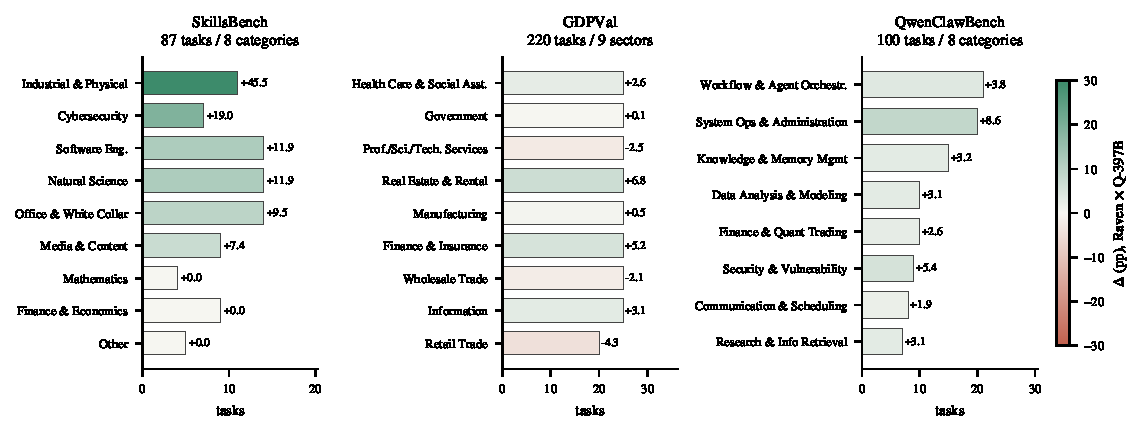
\includegraphics[width=\textwidth]{figures/fig_domain_coverage.pdf}
\caption{Cross-benchmark domain coverage of the evaluation, each
panel in its benchmark's native taxonomy.}
\label{fig:domain_coverage}
\end{figure*}

At the task level, the relevance of the best-retrieved skill
predicts the gain more directly than these coarse domain bins.
Beyond the binned summary in the main text
(Figure~\ref{fig:coverage-binned}), Figure~\ref{fig:coverage} plots
each SkillsBench task's $\Delta$ against the top reranker score of
its best-matched skill, a proxy that reflects both whether the
corpus holds a matching skill and whether retrieval surfaces it.
The positive slope holds across all four cells (Pearson
$r{=}0.31$--$0.40$, all $|t|{>}2.9$, $n{=}83$), the panel showing the
strongest cell.  The score is essentially uncorrelated with the
no-skill baseline ($|r|<0.05$), so partialling out task difficulty
leaves the association unchanged (partial $r{=}0.34$--$0.40$).

\begin{figure}[!ht]
\centering
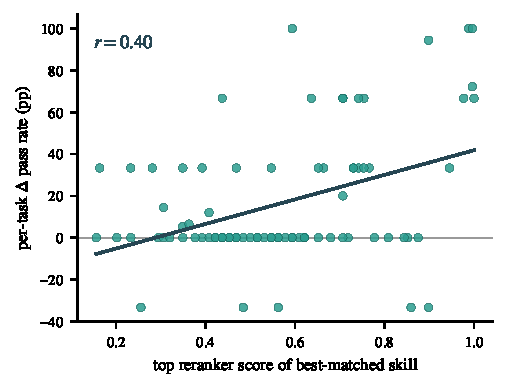
\includegraphics[width=0.86\columnwidth]{figures/fig_coverage.pdf}
\caption{Per-task SkillsBench gain versus corpus coverage
(top reranker score of the best-matched skill),
Raven~$\times$~Q-397B ($n{=}83$, $r{=}0.40$).}
\label{fig:coverage}
\end{figure}

% =============================================================================
\subsection{Class-Benchmark Alignment}
\label{app:class-bench-align}

\noindent Table~\ref{tab:class-bench-align} reports the
per-benchmark class over-selection underlying the class-adaptive
selection result of \S\ref{sec:claim-a}.  For each benchmark it
lists the skill classes most over-represented in the post-gate
selected pool relative to their corpus-wide frequency, showing
that each concentrates the gate on a different, task-appropriate
set of classes.  All three reject the null of the same class
distribution as the corpus (Pearson $\chi^2$ goodness-of-fit,
$p<10^{-10}$).

\begin{table}[!ht]
\centering\small
\setlength{\tabcolsep}{4pt}
\begin{tabular}{@{}lp{0.62\columnwidth}@{}}
\toprule
Benchmark & Over-selected classes (post-gate \% vs corpus \%) \\
\midrule
SkillsBench   & \textsc{Data} (38 vs 14), \textsc{Doc-Proc} (13 vs 3), \textsc{Security} (6 vs 4) \\
GDPVal        & \textsc{Writing} (31 vs 8), \textsc{Data} (29 vs 15), \textsc{Workflow} (14 vs 5) \\
QwenClawBench & \textsc{DevOps-Infra} (13 vs 8), \textsc{Meta} (11 vs 4), \textsc{Testing} (10 vs 6) \\
\bottomrule
\end{tabular}
\caption{Per-benchmark 16-class over-selection relative to the
corpus-wide baseline.}
\label{tab:class-bench-align}
\end{table}

% =============================================================================
\subsection{Case Studies: a Rescue and a Break}
\label{app:case-study}

We illustrate the end-to-end pipeline with two worked examples,
one task that skills rescue and one of the rare tasks that
skills break.  The rescue is
\texttt{manufacturing-\allowbreak codebook-\allowbreak normalization}, a SkillsBench
industrial-physical-systems task that the frontier check of
\S\ref{sec:frontier} (Claude~Opus~4.7 on the OpenClaw harness)
fails without skills and passes with them.

\paragraph{Task.}
Normalise free-form defect-reason texts from manufacturing test
logs (typos, abbreviations, mixed-language fragments) into a
standardised codebook: segment each raw text, assign a valid
code per segment subject to per-station code validity, and emit
calibrated confidence scores that distinguish \textsc{Unknown}
from low-evidence known predictions.

\paragraph{Retrieved skills.}
The gate (\S\ref{sec:retrieval}) selects two skills from the
corpus: a domain skill,
\texttt{manufacturing-\allowbreak failure-\allowbreak reason-\allowbreak codebook-\allowbreak normalization},
and a generic utility, \texttt{fuzzy-match}.  The domain skill's
body specifies the procedure rather than the topic:

\begin{quote}\small
``If \texttt{entry.stations} is not \texttt{None}, the predicted
code should only be considered valid when the record station
matches [\ldots] otherwise the code should be rejected.
[\ldots] consider multiple evidence sources [\ldots] (overlap or
fuzzy similarity between \texttt{span\_text} and codebook text
[\ldots], station compatibility, \texttt{fail\_code} alignment,
\texttt{test\_item} alignment, and conflict cues), and normalise
the score to a stable range $[0.0, 1.0]$.''
\end{quote}

\paragraph{Without skills.}
The agent writes a plausible solution built on a hard-coded
phrase dictionary with station filtering, but no multi-evidence
scoring and no confidence calibration.  It passes $15$ of $16$
verifier tests and fails the semantic-alignment check.  Only
$66.2\%$ of its non-\textsc{Unknown} predictions carry
non-trivial lexical evidence against the codebook (the verifier
requires $\geq 70\%$), i.e.\ it confidently emits codes the text
does not support.  Binary task reward: $0$.

\paragraph{With skills.}
The agent implements the skill's procedure directly:
multi-evidence weighted scoring, station-scope penalties, a
deterministic tie-break for near-tied candidates, and
calibrated confidence with an explicit \textsc{Unknown} band.
All $16$ tests pass, with $19\%$ less wall-clock time and
$20\%$ fewer total tokens than the failing no-skill run.

\paragraph{The break: \texttt{exceltable-in-ppt}.}
The complementary failure mode appears on one of the two tasks
the strongest open cell (Raven~$\times$~Q-397B) breaks
(no-skill passes, with-skill fails).  The task is to update an
exchange rate inside an Excel table embedded in a
PowerPoint slide, preserving its formulas.  Without skills the
agent improvises a working path through the four-layer
nesting, from the PPTX part through the OLE blob and its
embedded ZIP down to the sheet XML, patches the cell, and
re-packs the blob ($8/8$ verifier
tests pass).  With skills, the gate injects two topically
relevant Office skills whose recipes all operate on
top-level files
(\texttt{load\_workbook("file.xlsx")},
\texttt{Presentation("file.pptx")}).  The agent follows the
recipes, hits an API wall
(\texttt{property 'blob' of '\_OleFormat' has no setter}), and
never replaces the embedded object.  The verifier reads
\texttt{nan} where the table should be ($6/8$).  The skills are
on-topic, but their procedures do not extend to this task's
structure, and having a recipe displaced the improvisation that
succeeds without one.

\paragraph{Takeaway.}
The rescue and the break are two sides of the same property.
Skills transfer procedures, not topics.  When the
injected procedure matches the task's structure, as with the
multi-evidence scoring formulas and tie-breaks above, it
supplies exactly what the model does not reliably improvise.
When it does not, as with flat-file recipes against an embedded
object, following it can displace an improvisation that would
have succeeded.  This
is also one concrete reason composite quality scores cannot
predict per-task outcomes (\S\ref{sec:claim-a}).  The skills in
both cases are well-crafted, and what differs is
procedure--task fit.

% #############################################################################
\section{Compute and Reproducibility}
\label{app:compute-repro}

% =============================================================================
\subsection{Per-Stage Compute}
\label{app:compute}

The ingest pipeline was served on an internal GPU cluster using
Qwen3.5-397B-A17B-GPTQ-Int4 as the LLM judge for quality
scoring, classification, and embedding-based dedup.  This judge
is an open-weight model, publicly available on Hugging Face and
via OpenRouter, so the quality, safety, and classification labels
can be re-derived independently.  The internal cluster refers only
to where we ran it.  The compute
reported below is the cumulative total over the crawl that
produces the released active set.

\paragraph{Ingest compute.}
The ingest pipeline issued approximately $269{,}000$ LLM-judge
calls in total: $101{,}111$ per-skill quality + 3-facet score
calls on the post-dedup survivors (one call per row of the
released \texttt{quality\_judgments} table), $101{,}111$
single-label 16-class classification calls on the same set,
and $66{,}751$ pair-wise dedup adjudication calls on the
borderline embedding-cosine near-duplicate pairs
(\S\ref{sec:pipeline}), per the released dedup report.  Calls were issued at standard worker concurrency
on an internal GPU cluster running
Qwen3.5-397B-A17B-GPTQ-Int4.  The LLM-judge stage dominates
wall time, while content-hash, length-gate, and licence-API stages run
at file-IO / network speed and contribute negligible compute.

\paragraph{Evaluation compute.}
The main grid comprises $24$ configurations ($2$ conditions
$\times$ $4$ cells $\times$ $3$ benchmarks), each run three
times, on the two open Q-27B and
Q-397B backbones, served through Volcano (and, for one cell of
OpenClaw, DashScope).  The Opus~4.7
frontier robustness check ($2$~conditions $\times$ $87$~SkillsBench
tasks $= 174$~task runs) consumed approximately $24$~million
API tokens in total, estimated from the per-task token counters
recorded in the released eval cache
(mean $158$K total tokens per task for the SkillCorpus condition
and $122$K for the no-skill baseline, $87$ tasks each).  The per-task safety-facet regression on
SkillsBench (\S\ref{sec:claim-a}) reuses traces from the main
grid and adds negligible incremental cost.  Aggregate
wall-clock and GPU-hour accounting per ingest pass and per
evaluation cell is provided in the released compute log
alongside the corpus artifact.

% =============================================================================
\subsection{Reproducibility}
\label{app:reproducibility}

The corpus artifact (SQLite database, embeddings, quality cache,
per-stage reject reports) and the ingest pipeline source will be
released upon acceptance, linked from a public Hugging~Face dataset
entry and a GitHub repository hosting the pipeline code under a
permissive licence.

\paragraph{Multi-run merge protocol.}
The released active set is the cumulative union of multiple
ingest passes over the same SQLite database.  Content-hash and
name-hash dedup operate
across all passes, so ingesting a repository whose skills are
content-identical to rows already in the database produces no
duplicate rows.  The released active set is the database snapshot
at release time restricted to rows with $\mathtt{active}=1$ and
$\mathtt{deleted}=0$, the canonical release predicate.  Per-pass
reject counts and the chronological sequence of pipeline
configuration deltas are preserved in the released ingest report.

\paragraph{Reproducing the release predicate.}
A consumer reproducing the released set from the SQLite database
applies the predicate $\mathtt{active}=1 \wedge \mathtt{deleted}=0$
to the \texttt{skills} table, which yields exactly $96{,}401$
rows.  All downstream tables (\texttt{quality\_judgments},
\texttt{source\_priors}, \texttt{vec\_skills}) are keyed on
\texttt{content\_hash} or \texttt{skill\_id} and join on the
released set.
